\documentclass{ctexart}
\usepackage{graphicx} % Required for inserting images
\usepackage{amsmath}
\usepackage{amssymb}
\usepackage{amsthm}
\usepackage{hyperref}
\usepackage{geometry}
\geometry{a4paper, left=1in, right=1in, top=1in, bottom=1in}
\usepackage{minted}

\title{《人工智能与机器学习基础》第二次实验报告}
\author{PB24000150 李欣宸}

\date{\today}

\begin{document}

\maketitle

\section{实验流程}

\begin{enumerate}
    \item 补全 \verb|submission.py| 中 PCA 和 GMM 聚类算法的代码实现;
    \item 运行了训练脚本,观察了降维效果的可视化图像;
    \item 书写代码以评判训练结果的 Davies-Bouldin 指数(DBI);
    \item 书写了枚举不同超参数组合的代码;
    \item 分析了不同超参数下可视化图像的差异及 DBI 指数的变化;
\end{enumerate}

\section{参数调整}

该实验中,我主要调整的参数是 \verb|pca_components|(PCA 降维后的维度)、\verb|gmm_max_iter|(GMM 聚类的最大迭代次数)和 \verb|gmm_tol|(用于判断收敛的阈值)。事实上,\verb|gmm_max_iter| 和 \verb|gmm_tol| 控制的量是相同的。

使 DBI 达到最小的参数组合是 \verb|gmm_max_iter=1, pca_components=9|。

经过我的分析,我大概可以得出如下的结论:

\begin{itemize}
    \item PCA 降维后的维度对聚类效果有显著影响,当维度为 $10$ 左右时,聚类效果最好;
    \item 对于本次实验,K-means 算法的 DBI 值最小,随着 GMM 的训练,DBI 越来越高(虽然单调性尚不明确);
\end{itemize}

我对每个参数的调整思路如下:

\subsection{PCA 降维后的维度}

我们发现,DBI 在维度非常小的时候($d\le 10$ 左右)随维度增高而下降;但当维度继续增高时,DBI 反而开始上升,如图 \ref{fig:dbi_vs_pca} 所示。

我对此做出的解释是,PCA 的前几个分量主要捕捉的是是数字的“模板”信息,而后面的分量主要捕捉的则是“频域”信息(如笔画的粗细、倾斜等)(见图 \ref{fig:eigenfaces});而模板信息的“距离”有意义,但频域信息的“距离”则不一定有意义,无法对 K-Means、GMM 等基于某种内积空间上“距离”的聚类算法提供有效的信息。随着维度的增高,噪声在数据中的占比越来越大,导致 DBI 反而上升。

\begin{figure}[htbp]
    \centering
    \includegraphics[width=0.9\textwidth]{imgs/dbi_vs_pca_by_tol.png}
    \caption{不同 PCA 降维维度下的 DBI 变化}
    此处 \verb|gmm_max_iter| 均为无穷大(即迭代次数只受 \verb|gmm_tol| 控制),\verb|gmm_reg_covar| 均设为 $10^{-6}$
    \label{fig:dbi_vs_pca}
\end{figure}


\begin{figure}[htbp]
    \centering
    \includegraphics[width=0.6\textwidth]{imgs/eigenfaces.png}
    \caption{PCA 前 64 个主成分可视化}
    从左到右、从上到下依次为第 $1$ 到第 $64$ 个主成分
    \label{fig:eigenfaces}
\end{figure}

\subsection{GMM 聚类的最大迭代次数与收敛阈值}

我们发现,DBI 随着最大迭代次数的增大而上升,也就是说,随着模型的训练,如果用 DBI 衡量聚类效果的话,模型的效果反而变差了,如图 \ref{fig:dbi_vs_gmm} 所示。

我对此的猜测是,Davies-Bouldin 指数衡量的是簇内距离与簇间距离的比值(见 \eqref{eq:dbi}),而 K-Means 算法的目标函数为 \eqref{eq:kmeans_obj};K-Means 更接近于“将所有欧式距离尽可能近的点划分到同一个簇中”,而 GMM 算法更倾向于根据数据点的分布情况,调整参数中的协方差矩阵,最大化真实数据的对数似然,并不会保证簇的形状尽可能接近球形;而在本题 DBI 恰恰是在 784 维的欧式空间中计算的,因此初始时的 DBI 反而比 GMM 训练后的 DBI 更小。

\begin{figure}[htbp]
    \centering
    \includegraphics[width=0.9\textwidth]{imgs/dbi_vs_iter.png}
    \caption{不同 GMM 最大迭代次数下的 DBI 变化}
    \label{fig:dbi_vs_gmm}
\end{figure}

\begin{gather}
    DBI = \frac{1}{k} \sum_{i=1}^{k} \max_{j \neq i} \left( \frac{s_i + s_j}{d_{ij}} \right)
    \label{eq:dbi} \\
    J = \sum_{i=1}^{k} \sum_{x \in C_i} \| x - \mu_i \|^2
    \label{eq:kmeans_obj}
\end{gather}

\section{实验效果}

下面我们展示 DBI 最低,以及充分收敛时的可视化图像。在本次实验中,DBI 最低的时候聚类效果并不好。在后面,我们分析三种降维方式的区别。

\subsection{DBI 最低时的可视化效果}

DBI 最低的参数组合是 \verb|gmm_max_iter=1, pca_components=9|,此时 DBI 值为 $2.8229$。\ref{fig:best_dbi} 分别展示了使用自编码器、PCA 和 t-SNE 降维后的可视化效果。

可以看出,在 PCA 降维后,GMM 算法得到的标签(其实可以看作 K-Means 后初始化的结果)中簇的形状更接近圆形(比如左侧的类别 $1$ 在右图中被拆分成类别 $7$ 和 $9$),这个聚类结果更符合 DBI 的计算方式,因此 DBI 更低

而 t-SNE 聚类的结果更符合真实标签,而不是 K-Means 初始化得到的标签,因此 DBI 反而更高(约为 $3.9629$)。

\begin{figure}[htbp]
    \centering
    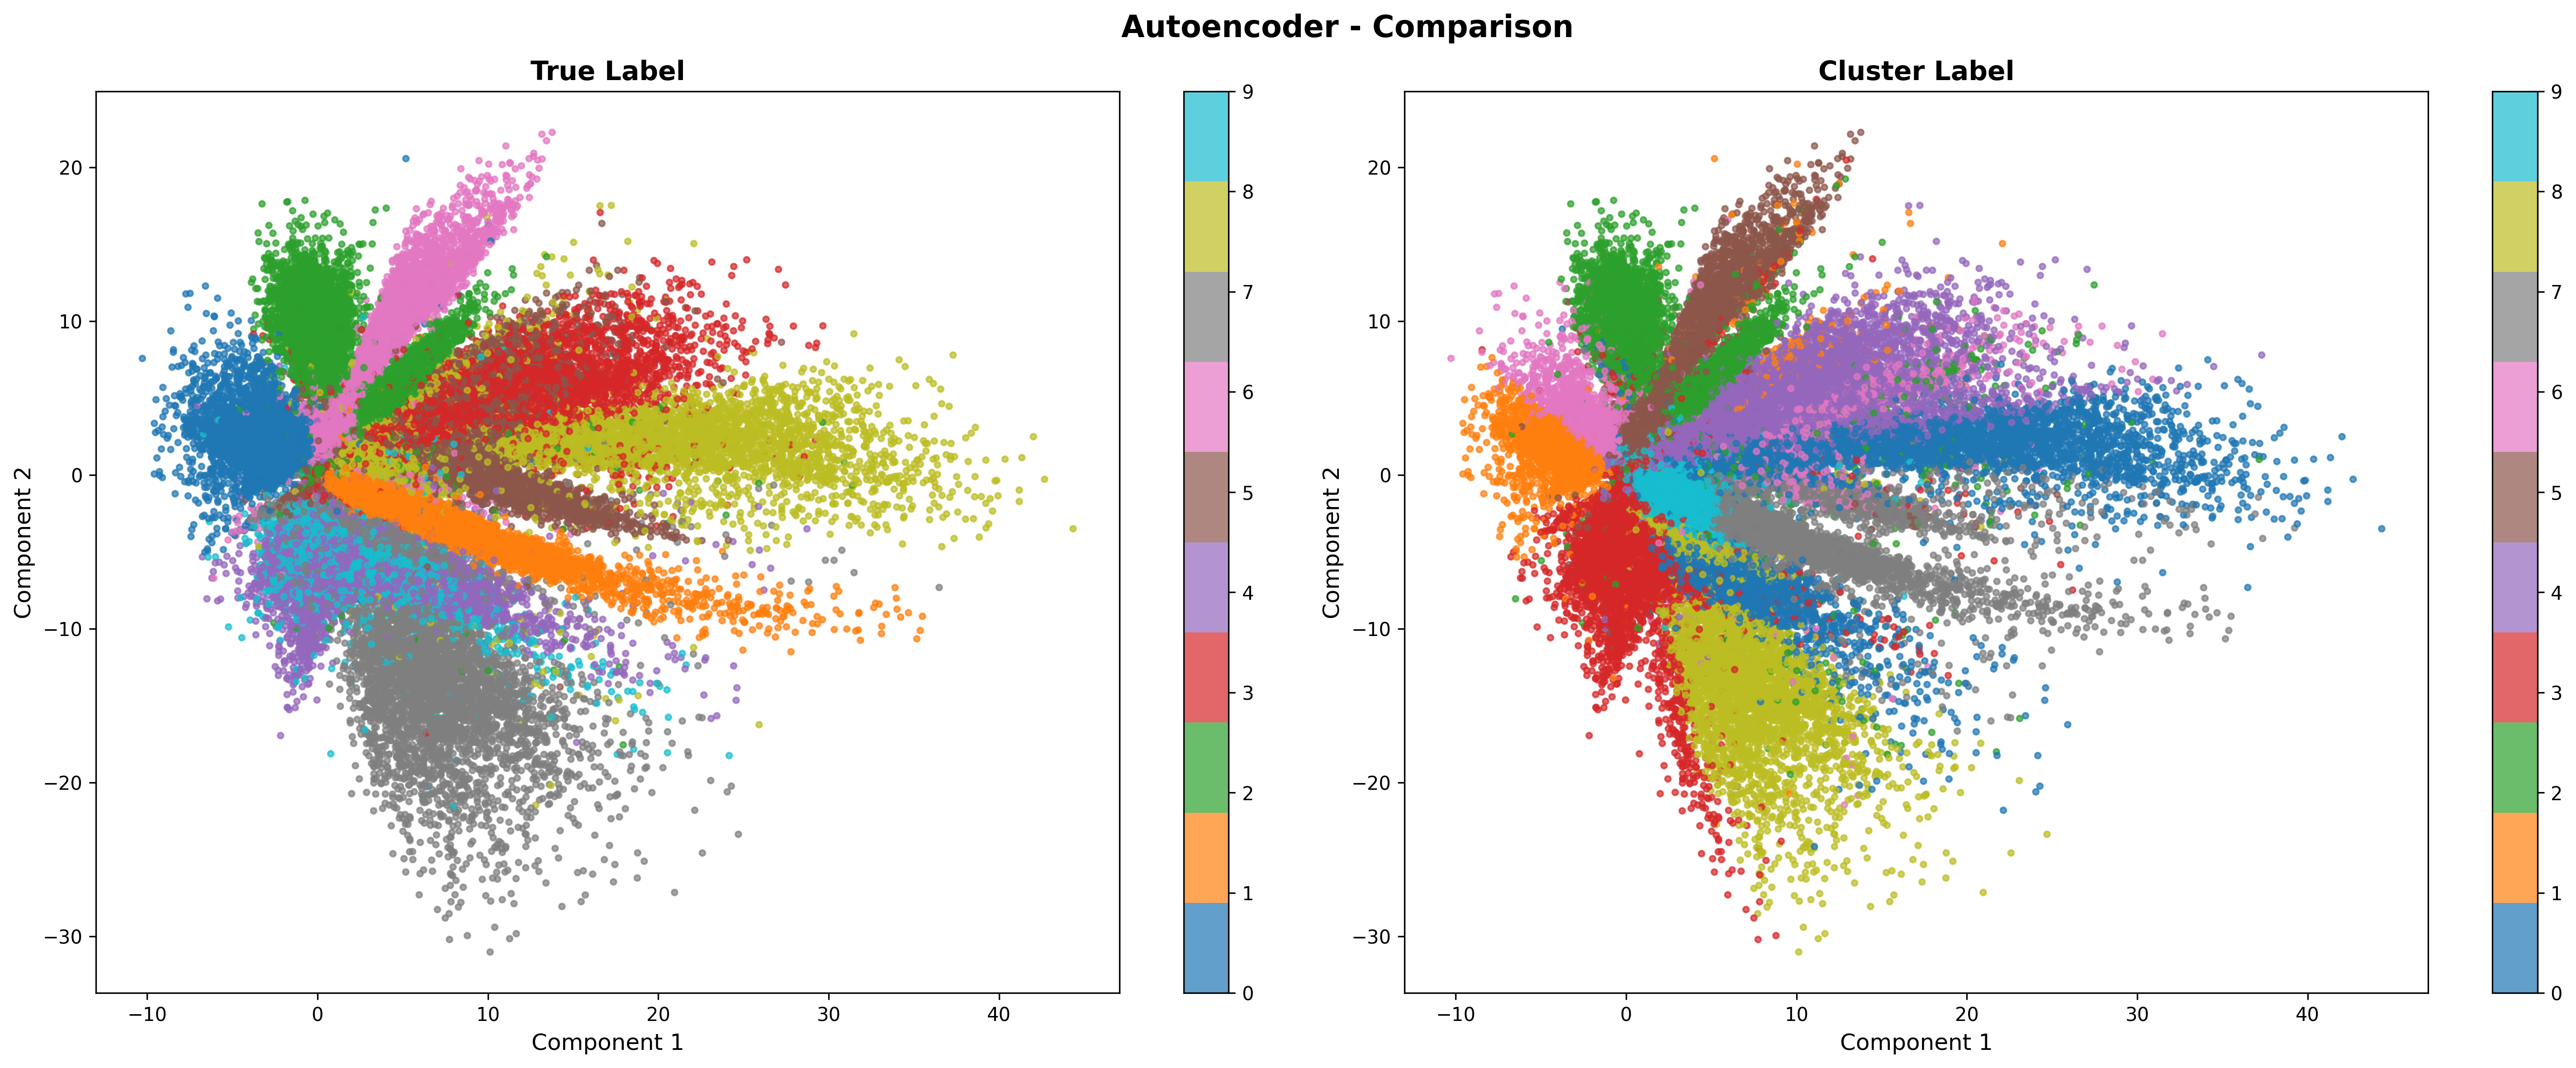
\includegraphics[width=0.97\textwidth]{imgs/best_dbi_ae.png}
    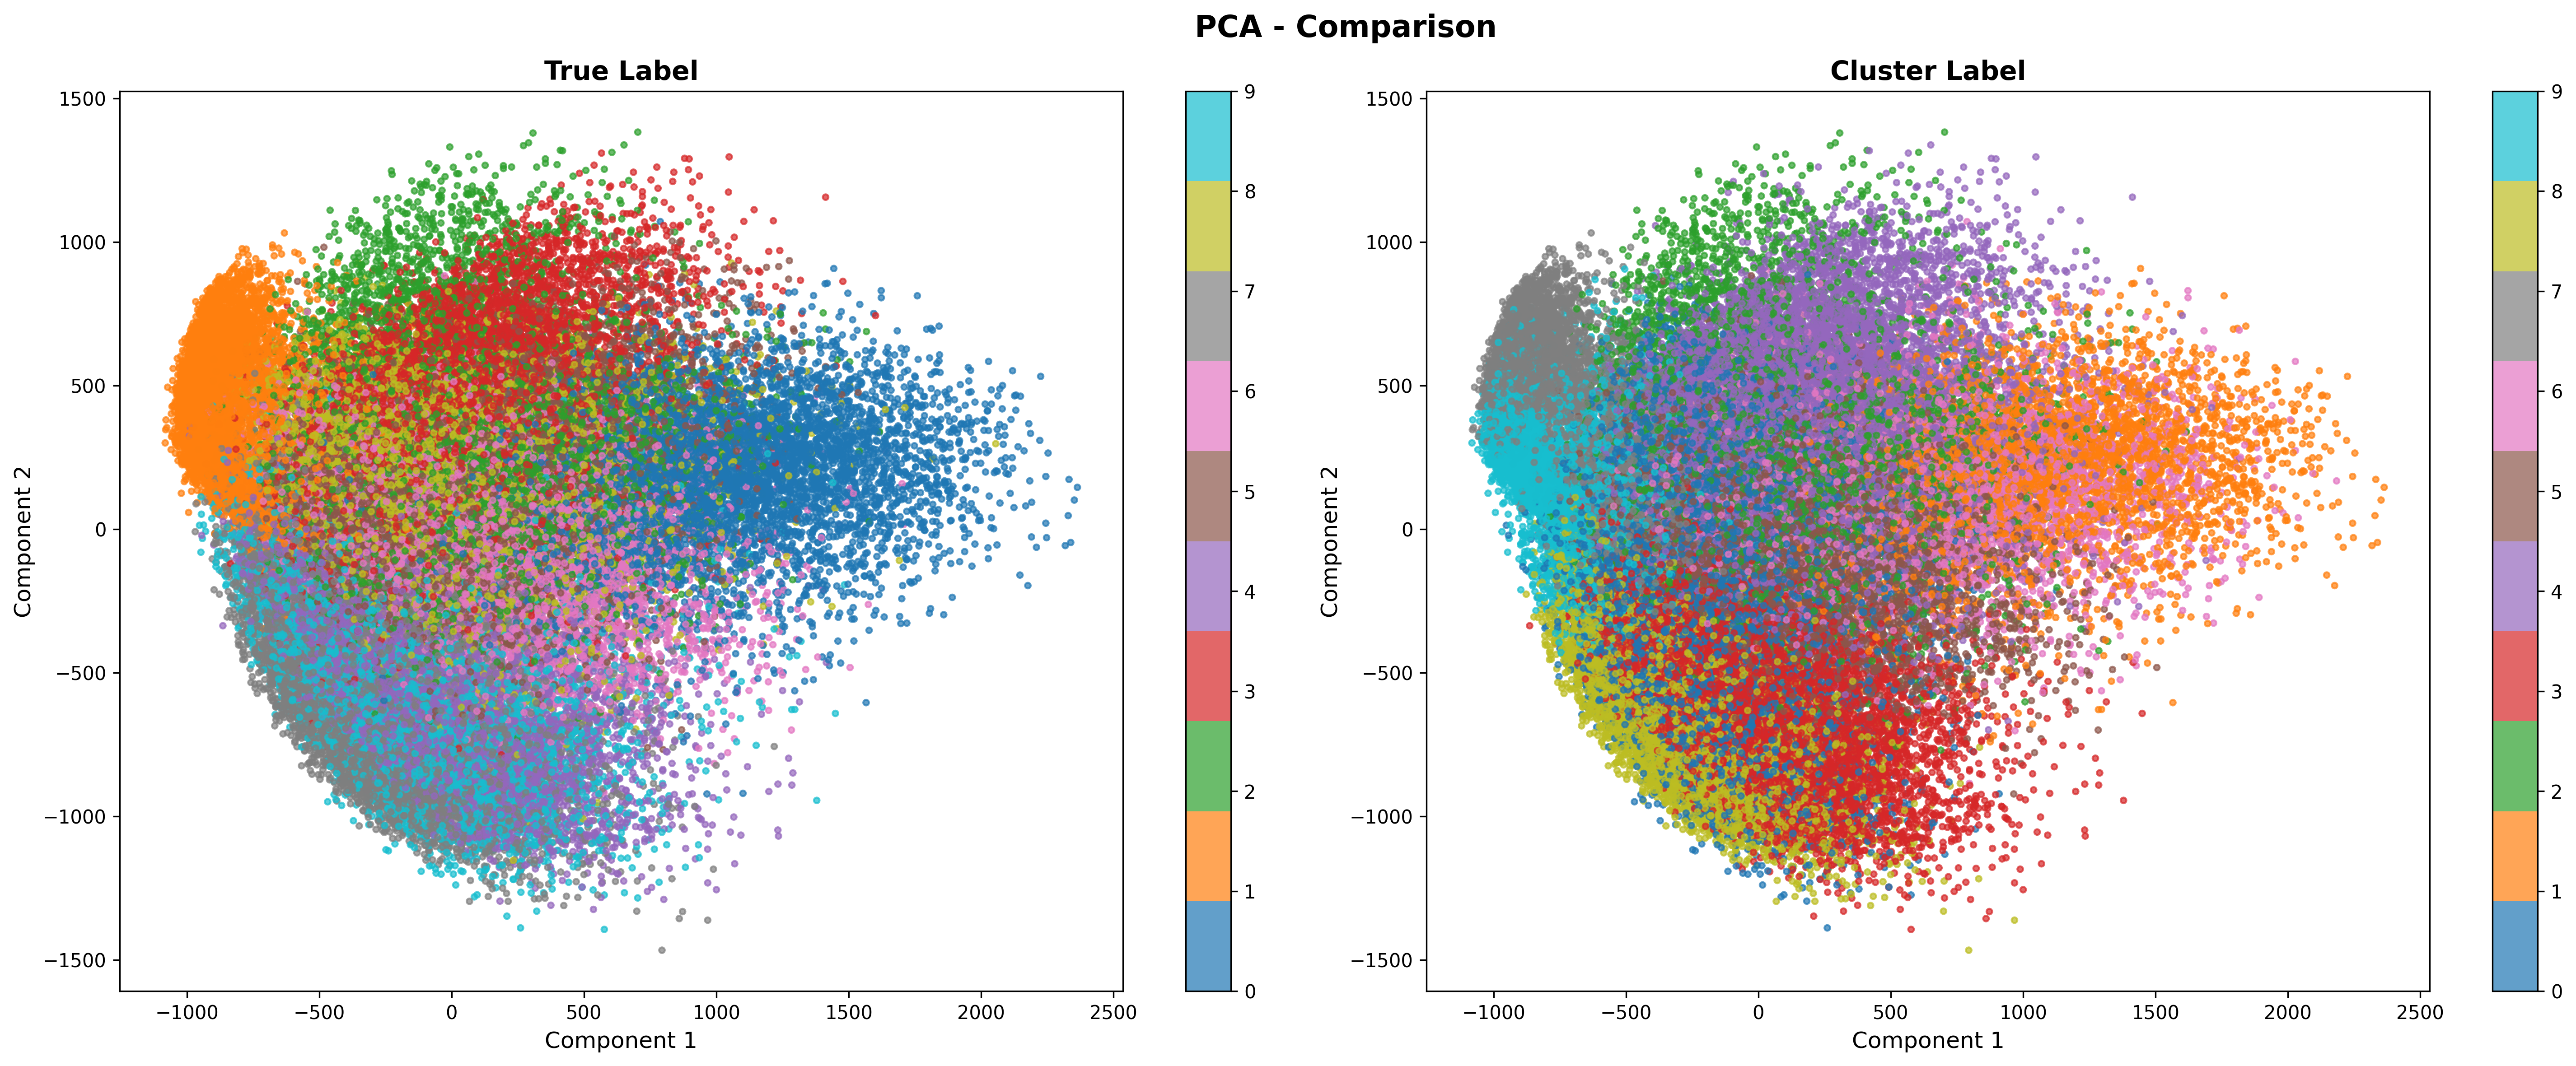
\includegraphics[width=0.97\textwidth]{imgs/best_dbi_pca.png}
    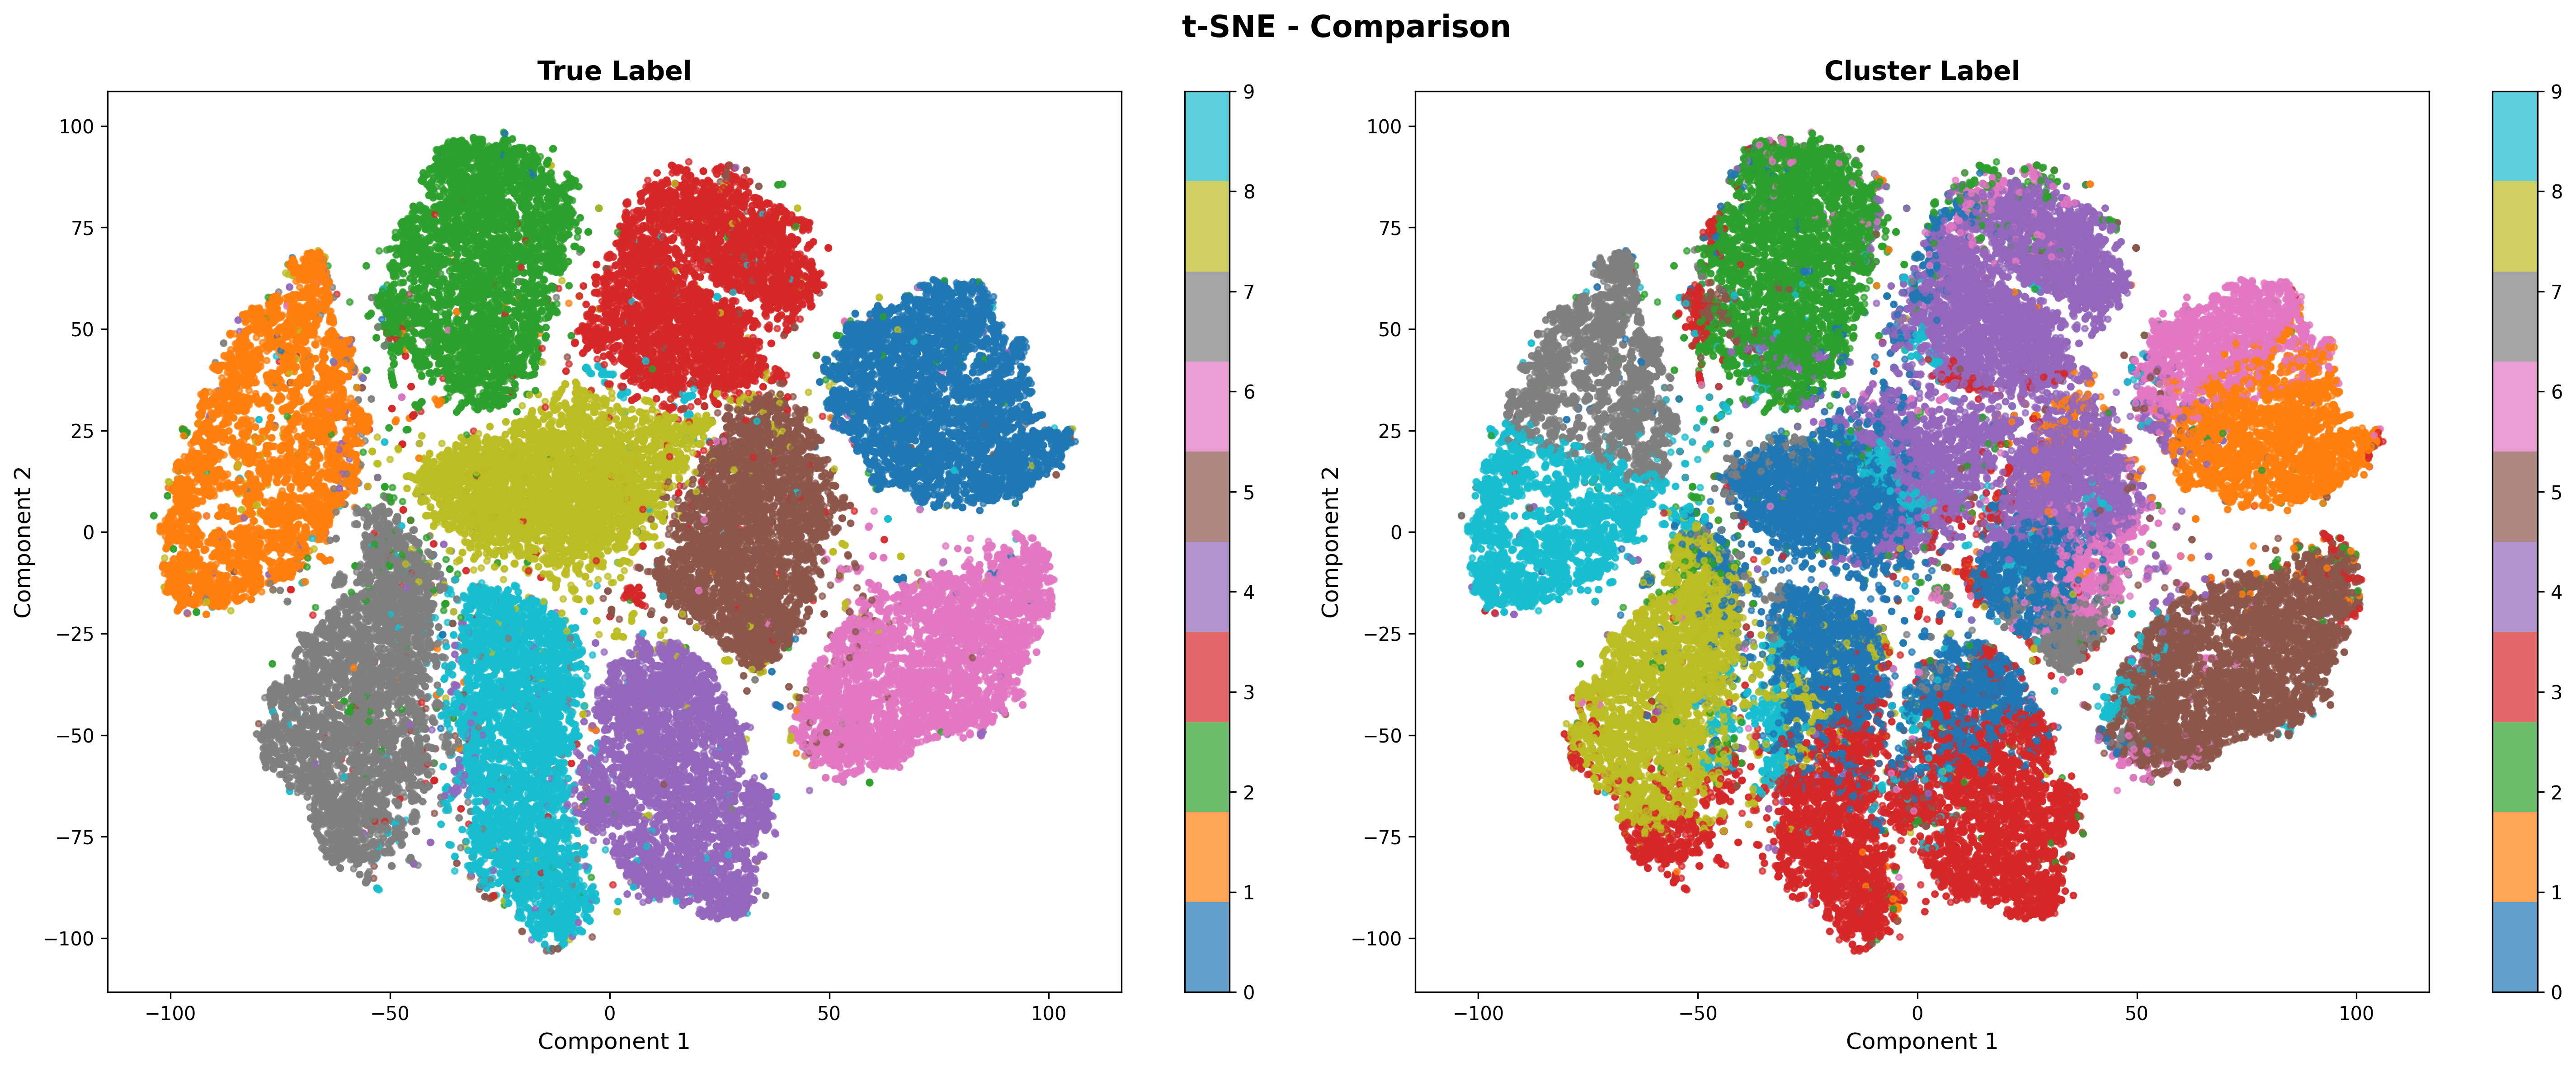
\includegraphics[width=0.97\textwidth]{imgs/best_dbi_tsne.png}
    \caption{DBI 最低时的可视化效果(从上到下依次为 Autoencoder、PCA、t-SNE)}
    可视化效果均使用 \verb|python visualization.py --results_path <checkpoint>| 命令生成。我对 \verb|visualization.py| 进行了一定的修改(缩小了数据点大小),以便更好地观察聚类效果。
    \label{fig:best_dbi}
\end{figure}

\subsection{充分收敛时的可视化效果}

GMM 充分收敛时(\verb|gmm_tol=1e-5, pca_components=10|)的可视化效果和充分收敛前没有明显差别,故省略此处展示,此时 DBI 值约为 $2.8519$,较充分收敛前略有增加。

\subsection{三种降维方式的比较} \label{sec:dim_reduction_compare}

\subsubsection{自编码器降维}

由于自编码器降维的目标是最大化重建数据的准确性,因此它能够保留更多的数据信息;本题中给出的编码器是普通自编码器,没有对隐变量的分布做任何假设,因此真实下标中簇的形状相对不规则。比如图 \ref{fig:best_dbi} 中,簇的形状比较类似放射状。

我们猜测,如果对隐变量的分布做出高斯混合的假设(即使用一种特殊的变分自编码器 GMVAE\footnote{可以参考 \url{https://arxiv.org/abs/1611.02648})},那么降维后的隐分布可视效果可能会更好。

\subsubsection{PCA 降维}

由于 MNIST 数据集有着极强的非线性特征,PCA 作为一种线性降维方法,无法很好地捕捉数据的非线性结构,因此在 \ref{fig:best_dbi} 中,PCA 降维后不同类别的数据点混杂在一起,无法很好地分离开来。

我们也可以从方差解释率的角度来理解 PCA 的不足,如图 \ref{fig:explained_variance} 所示。可以看到,前 $2$ 个(即用于可视化的维度)主成分只贡献了 $16.80\%$ 的方差解释率,无法囊括用于区分数字类别的足够信息是正常的。

\begin{figure}[htbp]
    \centering
    \includegraphics[width=0.8\textwidth]{imgs/cumulative_variance.png}
    \caption{PCA 前若干个主成分的累计方差解释率}
    \label{fig:explained_variance}
\end{figure}

\subsubsection{t-SNE 降维}
相比之下,t-SNE 降维的形状更加规则,由图 \ref{fig:best_dbi} 可以看出,不同类别的数据点都聚集在形状接近圆形的簇中,簇与簇之间的间隙较小,像若干到沟壑把平面分割为若干个“区块”。

这可以从 t-SNE 主要保留局部结构的角度来理解。

\section{思考题}

\subsection{先降维后聚类的原因}

先降维后聚类的原因主要有以下几点:

\begin{enumerate}
    \item \textbf{维度灾难}:高维数据空间中,数据点之间欧氏“距离”的意义会变得模糊;降维可以减少维度灾难的影响,使得距离度量更加有效;
    \item \textbf{去除噪声}:高维数据中往往包含大量噪声和冗余信息,降维有助于保留有效信息,去除无关信息,提高聚类的准确性;
    \item \textbf{计算效率}:数据的维度越高,计算时间越长;降维可以显著减少计算时间;
    \item \textbf{可解释性}:低维空间更容易进行可视化和解释,训练出的模型更简单,更具可解释性;
\end{enumerate}

\subsection{降维方法的区别}

结合实验具体数据的分析见 \ref{sec:dim_reduction_compare},下面是大概的比较:

\begin{itemize}
    \item \textbf{训练速度}:PCA 的时间复杂度为 $\mathcal{O}(nd^2 + d^3)$,其中 $n$ 是样本数量,$d$ 是特征维度;Barnes-Hut 优化的 t-SNE 的时间复杂度为 $\mathcal{O}(T (n \log n + nd))$,其中 $T$ 是迭代次数;由于 t-SNE 算法中有梯度下降的过程,所以其训练速度通常比 PCA 慢很多;
    \item \textbf{降维效率}:在\textbf{推理}过程中,PCA 的时间复杂度为 $\mathcal{O}(dk)$,其中 $k$ 是降维后的维度;Autoencoder 是神经网络模型,推理的时间复杂度取决于网络结构和层数;它们都是参数化模型,在训练完成后可以处理新的数据点,而 t-SNE 不是参数化模型,无法直接对新数据进行降维;
    \item \textbf{灵活性}:PCA 的超参数只有维度 $k$;t-SNE 有多个超参数,如学习率、迭代次数、困惑度等,可以根据数据集进行调整;而 Autoencoder 的结果和超参数的选择(如网络结构、激活函数、正则化方法等)密切相关,具有极高的灵活性;
    \item \textbf{数据分布保持程度}:PCA 是正交变换,能保留数据的全局线性结构,降维后的距离也能很好地反映原始空间中的距离关系;t-SNE 更关注局部结构,能更好地保留数据点之间的局部邻近关系,但可能会扭曲全局结构;Autoencoder 的表现取决于网络结构和训练过程,可能在某些情况下既能保留局部结构,也能保留全局结构,但不保证一定如此;
    \item \textbf{可视化效果}:PCA 对于非线性可分数据的可视化效果一般较差;相比之下,t-SNE 和 Autoencoder 的可视化效果一般较好。
\end{itemize}

\subsection{K-Means 与 GMM 的异同}

\begin{itemize}
    \item \textbf{相同点}:
    \begin{itemize}
        \item 都是无监督学习中的聚类算法;
        \item 都假设数据点是由多个簇组成的,每个簇由一个中心点(K-Means)或一个概率分布(GMM)表示;
        \item 都使用 EM 算法进行参数估计和簇分配;K-Means 可以看作 GMM 在先验概率相同,协方差矩阵为单位矩阵乘以一个无穷小量时的特例;
        \item 初始化对算法执行效果的结果影响较大,通常采用随机重启等方法以获得更好的结果。
        
    \end{itemize}
    \item \textbf{不同点}:
    \begin{itemize}
        \item K-Means 假设每个簇是球形的,且簇内数据点服从均匀分布;而 GMM 假设每个簇服从高斯分布,可以表示更复杂的簇形状;
        \item K-Means 使用硬分配方法,每个数据点被分给唯一的一个簇;而 GMM 使用软分配方法,计算每个数据点属于每个簇的概率;
        \item K-Means 与 GMM 的目标函数不同,K-Means 最小化簇内平方误差,而 GMM 最大化数据的证据下界。
    \end{itemize}
\end{itemize}

\section{课程反馈}

\subsection{花费时间}

我在本次实验中大概花费了 12 到 16 个小时完成全部内容,主要时间花费在意识到 DBI 指数低与标签更接近真实标签的区别上。

\subsection{建议}

在 GMM,K-means 算法的学习中,选择簇的数量是一个重要的问题。希望实验中能训练同学们如何使用不同的方法(如肘部法则、轮廓系数等)来确定最佳簇数量。

希望将来该课程的 GMM 实验的主题能更加贴近该算法实际应用场景,例如语音识别(GMM 对 MFCC 特征建模)等,而不是用其他领域中的数据集代替,使同学们能更好地理解该算法的应用价值和效果。

\end{document}
